\section{Adversarial tree search}
\label{sec:theory}

Consider a deterministic zero-sum two-player game as a 4-tuple $G = (S, A, R, U)$, where $S$ is the set of all states, $A$ is the set of all actions, some of which may not be applicable in some states and $R: S \times A \rightarrow S$ is the transition function describing the result of taking a certain action in a certain state. Let $S^\circ \subset S$ be the set of all terminal states, then $U: S^\circ \rightarrow \mathrm{R}$ is the utility function associating each terminal state with a real number. Since not all actions are applicable in all states, let $A(s) \subseteq A$ denote the subset of actions that are applicable in the state $s$. The set $S'(s) = \{ R(s, a) \; | \; a \in A(s) \}$ contains the successor states of $s$, which are all states reachable from $s$ by taking an applicable action.

To enforce the zero-sum property, the first player to take action will recieve a utility of $U(s)$ in terminal states, while the second player recieves $-U(s)$. The first player will be reffered to as the Max player, and the second as the Min player, as they seek to respectively maximize and minimize the utility function.

The question is now, given a state $s_0 \in S$, what action should a rational agent take? To answer this question, we model the game as a game tree, starting with a root node containing the current state $s_0$. Each node in the game tree has a set of children, containing one child node for each state in $S'(s)$:

\begin{figure}[H]
    \centering

    \tikzset{
    max node/.style={circle,draw,inner sep=5},
    min node/.style={circle,draw,inner sep=5, fill=gray}
    }

    \begin{tikzpicture}[scale=12]
    % Specify spacing for each level of the tree
    \tikzstyle{level 1}=[level distance=1.7mm,sibling distance=4mm]
    \tikzstyle{level 2}=[level distance=1.7mm,sibling distance=2mm]
    % The Tree
    \node(0)[max node]{$s_0$}
    child{node(1)[min node]{$s_1$}
        child{node[max node, label=below:{$U(s_3)=1$}]{$s_3$}
            edge from parent node[left]{$a_0$}
        }
        child{node[max node, label=below:{$U(s_4)=-1$}]{$s_4$}
            edge from parent node[right]{$a_1$}
        }
        edge from parent node[left]{$a_0$}
    }
    child{node(2)[min node]{$s_2$}
        child{node[max node]{$s_5$}
            child{node[min node, label=below:{$U(s_6)=0$}]{$s_6$}
                edge from parent node[left]{$a_0$}
            }
            child{node[min node, label=below:{$U(s_4)=-1$}]{$s_4$}
                edge from parent node[right]{$a_1$}
            } 
            edge from parent node[right]{$a_0$}
        }
        edge from parent node[right]{$a_1$}
    };

    \end{tikzpicture}

    \caption{A simple game tree where white nodes correspond to the
    Max player's turn, and grey nodes to the Min player's. Notice how
    not all actions are applicable in all states, terminal states do
    not have to be on the same depth, and a given terminal state will have
    the same utility regardless of the path leading to it.}
    \label{fig:game_tree}

\end{figure}


In the game from Figure \ref{fig:game_tree}, it is easy to see that in order to maximize the utility function, the Max player should take action $a_1$, forcing the Min player into action $a_0$, and then taking $a_0$ for a utility of $0$. While a higher utility is available in the subtree stemming from first taking $a_0$, an optimal Min player would pick $a_1$ every time, leading to a worse outcome for Max.

While it is easy to see these optimal decisions in a small game tree, even Tic Tac Toe has a game tree complexity (the number of leaf nodes in the game tree) on the order of $10^5$, while games like Chess and Go reach $10^{123}$ and $10^{360}$ respectively. Trees of these sizes are currently impossible to search completely, so in order to construct a game playing agent based on tree search methods, it is necessary to reduce the amount of nodes that needs to be searched.

\subsection{MiniMax}

As the classical approach to adversarial search, MiniMax builds on the idea of minimizing the maximum amount of utility that your opponent can achieve, in other words making their optimal choice as bad as possible. The MiniMax value of a state can be recursively defined as

\begin{equation}
    MiniMax(s) = \begin{cases}
        U(s) & s \in S^\circ \\
        \max_{a \in A(s)} MiniMax(R(s, a)) & Player(s) = Max \\
        \min_{a \in A(s)} MiniMax(R(s, a)) & Player(s) = Min
    \end{cases}
    \label{eq:MiniMax}
\end{equation}
where $Player(s)$ returns the player which turn it is to take action in state $s$. From this optimal play can be achieved by following the policy given by:
\begin{equation}
    TakeAction(s) = \begin{cases}
        \arg\max_{a \in A(s)} MiniMax(R(s, a)) & Player(s) = Max \\
        \arg\min_{a \in A(s)} MiniMax(R(s, a)) & Player(s) = Min
    \end{cases}
    \label{eq:MiniMax_policy}
\end{equation}
This means that optimal play for the Max player simply consists of choosing the action which leads to the state with the highest MiniMax value, and vice versa for the Min player. Take the game tree from Figure \ref{fig:game_tree} as an example:

\input{tikz/MiniMax_example.tex}

\input{algorithms/MiniMax}

The pseudocode of a pure MiniMax algorithm can be seen in Algorithm \ref{alg:minimax}. If MiniMax is implemented as shown, a Depth First Search (DFS) with added backup of the MiniMax values, it has a time complexity of $\mathcal{O}(b^m)$ and a space complexity of $\mathcal{O}(m)$, where $b$ is the average number of applicable actions, also called the branching factor, and $m$ is the depth of the deepest node in the game tree. Most notably however, is that it searches the \textit{entire} game tree, making it intractable for the vast majority of games.

Many methods exist to make MiniMax practical on large game trees, three of which will be introduced in this paper: $\alpha\beta$-pruning, iterative deepening, and Best First MiniMax.  The first two methods are by far the most widely used, and most if not all modern MiniMax agents implement both.

\subsubsection{AlphaBeta-pruning}
This is a quick introduction, for a more in depth explanation see \cite[p. 198]{russellnorvig}.
$\alpha\beta$-pruning can be thought of as a simplification of the MiniMax formula that is applicable in certain cases, and as such it still guarantees optimality. Consider the following example:
\begin{align*}
    MiniMax(s) &= \max(MiniMax(R(s, a_0)), MiniMax(R(s, a_1)), 
    MiniMax(R(s, a_2))) \\
    &= \max(\min(5, 12, 8), \min(x_0, 1, x_1), \min(12, x_2, 4)) \\
    &= \max(5, y_0, y_1), \;\; y_0 \leq 1, \; y_1 \leq 4 \\
    &= 5
\end{align*}
On the second line some values are missing, but the values that are present can be used to set an upper bound for their corresponding $\min$ statements, which in turn can be used to determine the value of the $\max$ statement. This method can be used all throughout the MiniMax algorithm, potentially cutting off huge subtrees from the search space, allowing it to search much deeper. Since the example is very shallow, it does not illustrate this to full effect, but if the actions are expanded in the optimal order, $\alpha\beta$-pruning has a time complexity of $\mathcal{O}(b^{m/2})$, which compared to MiniMax's $\mathcal{O}(b^{m})$ lets $\alpha\beta$-pruning search twice as deep in the same time. In practice the actions cannot be expanded in the optimal order since an optimal ordering could be used to play the game optimally, but existing methods can get quite close to the theoretical limit \cite[p. 201]{russellnorvig}.


\begin{algorithm}[H]
    \caption{Depth Limited Minimax with $\alpha\beta$-Pruning}
    \label{alg:alphabeta}
    \begin{algorithmic}[1]
    
    \Procedure{Alpha-Beta}{$s$, $d$}
        \State \Return $\arg\max_{a \in A(s)}$ Min-Value(R(s, a))
    \EndProcedure
    \end{algorithmic}

    \begin{algorithmic}[1]

    \Procedure{MaxValue}{$s$, $\alpha$, $\beta$, $d$}
        \If{$s \in S^\circ$ \textbf{or} $d=0$}
            \Return $E(s)$
        \EndIf
        \State $v \leftarrow -\infty$
        \For{$a \in A(s)$}
            \State $v \leftarrow \max(v, MinValue(R(s, a), \alpha, \beta, d-1))$
            \If{$v \geq \beta$}
                \Return $v$
            \EndIf
            \State $\alpha \leftarrow \max(\alpha, v)$
        \EndFor
        \State \Return $v$
    \EndProcedure
    
    \end{algorithmic}
        
    \begin{algorithmic}[1]

    \Procedure{MinValue}{$s$, $\alpha$, $\beta$, $d$}
        \If{$s \in S^\circ$ \textbf{or} $d=0$}
            \Return $E(s)$
        \EndIf
        \State $v \leftarrow \infty$
        \For{$a \in A(s)$}
            \State $v \leftarrow \min(v, MaxValue(R(s, a), \alpha, \beta, d-1))$
            \If{$v \leq \alpha$}
                \Return $v$
            \EndIf
            \State $\beta \leftarrow \min(\beta, v)$
        \EndFor

        \State \Return $v$
    \EndProcedure

    \end{algorithmic}
\end{algorithm}
\subsubsection{Iterative Deepening}
Iterative deepening builds on depth limited search, which as the name suggests terminates the recursion at a predetermined depth instead of continuing to a terminal state. However, from the definition of games in the beginning of this section it is clear that only terminal states have a utility value, so the algorithm has nothing to return if recursion stops earlier. To overcome this issue, an evaluation function $E: S \rightarrow \mathbb{R}$ is introduced, representing an estimate of the true game theoretical value of the position. This evaluation function can be based on domain knowledge e.g. in chess it could be piece values and positioning principles, it can be learned using neural networks, or it can be a combination of both. A depth limited search of depth $d$ has a time complexity of $\mathcal{O}(b^d)$ and a space complexity of $\mathcal{O}(d)$,since it forces the deepest node in the tree to have depth at most $d$. Since the algorithm no longer searches the entire game tree and uses an approximation for the MiniMax value at cutoff nodes, it is no longer guaranteed optimal, but can still produce strong play with a good evaluation function.

Having the ability to limit the search to a certain depth is a great improvement, but it can still be difficult to estimate how much time a search to a given depth will take, which is a problem in most applications. Iterative deepening overcomes this issue by starting at depth limit $d=1$, which is guaranteed to complete almost instantly, storing the best move, increasing the depth limit to  $d=2$, and so on. This way when time runs out the algorithm will always have an action to return. The main concern about iterative deepening is that the algorithm has to search many nodes multiple times, thereby wasting time. While this is true, the amount of re-searched nodes is much smaller than one might think, since the exponential nature of game trees make shallower levels of the tree much smaller than deeper ones. Take a game with branching factor $b=10$, searched to depth $d=5$. A normal depth limited search would search $10^1+10^2+10^3+10^4+10^5=111,110$ nodes, while an iterative deepening search would search $5 \cdot 10^1+4 \cdot 10^2+3 \cdot 10^3+2 \cdot 10^4+10^5=123,450$ nodes, which is only an $11.11\%$ increase \cite[p. 99]{russellnorvig}. If combined with $\alpha\beta$-pruning, iterative deepening can even decrease the number of nodes searched by improving move ordering.

\begin{algorithm}[H]
    \caption{Iterative Deepening Minimax}
    \label{alg:iterativedeepening}
    \begin{algorithmic}[1]
    
    \Procedure{Iterative-Deepening}{$s$}
        \State $d \leftarrow 1$
        \While{\textbf{not} SearchTimeExhausted()}
            \State $Action \leftarrow \arg\max_{a \in A(s)}$ MinValue($R(s, a)$, $d - 1$)
            \State $d \leftarrow d + 1$
        \EndWhile
        \State \Return $Action$
    \EndProcedure
    \end{algorithmic}

    \begin{algorithmic}[1]

    \Procedure{MaxValue}{$s$, $d$}
        \If{$s \in S^\circ$ \textbf{or} $d=0$}
            \Return $E(s)$
        \EndIf
        \State $v \leftarrow -\infty$
        \For{$a \in A(s)$}
            \State $v \leftarrow \max(v, \text{MinValue}(R(s, a), d-1))$
        \EndFor
        \State \Return $v$
    \EndProcedure
    
    \end{algorithmic}
        
    \begin{algorithmic}[1]

    \Procedure{MinValue}{$s$, $\alpha$, $\beta$, $d$}
        \If{$s \in S^\circ$ \textbf{or} $d=0$}
            \Return $E(s)$
        \EndIf
        \State $v \leftarrow \infty$
        \For{$a \in A(s)$}
            \State $v \leftarrow \min(v, \text{MaxValue}(R(s, a), d-1))$
        \EndFor

        \State \Return $v$
    \EndProcedure

    \end{algorithmic}
\end{algorithm}

\subsubsection{Best First MiniMax}
The classical approach to implementing MiniMax is via DFS, since it can compute the MiniMax move using linear space, and only needs to back up the MiniMax values once per state $\alpha\beta$-pruning and iterative deepening makes it possible to search less nodes and terminate early, but it is still only using information from the deepest nodes to guide the search. Best First MiniMax seeks to improve this by continually expanding the most promising nodes until a time or space limit is reached resulting in a tree with non-uniform depth.

In a non-adversarial setting, Best First Search uses a priority queue based frontier to determine which node to expand next, but that approach is difficult to transfer directly to adversarial search since nodes with high evaluation should have a high chance of leading to a win, but without searching the low evaluation nodes the agent does not see the refutations or even losing moves that an otherwise promising strategy might contain. Even if the frontier prioritized both extremes of the evaluation function, the average evaluation nodes still need to be explored in order to find possible extreme values in their subtrees. All this means that if the agent is not searching to a uniform depth, it needs a way to balance exploitation (expanding promising nodes) and exploration (expanding not so promising nodes).

The mechanism used by Best First MiniMax \cite{Korf1996} to achieve this balance is the principal variation, which is illustrated on Figure \ref{fig:minimax_example}. As seen in the figure, the principal variation is the path from the root to a leaf where all nodes have the same MiniMax value, ie. the leaf is  where the MiniMax value of the root stems from. This means that the root needs a MiniMax value in order for the principal variation to exist, and Best First MiniMax therefore has to back up MiniMax values on each iteration, which is the price it pays to achieve non-uniform expansion. The algorithm runs three steps over and over:
\begin{enumerate}
    \item Select the leaf at the end of the principal variation
    \item Fully expand this leaf
    \item Back up new MiniMax values 
\end{enumerate}
A common concern is that this would lead the algorithm to go down one promising path and never come back. This is not what happens, due to what the authors call the tempo effect. The tempo effect states that when expanding a max node the value tends to go up due to it taking on the maximum value of its children. This makes it less attractive to its parent min node, which decreases the chance that the max node will be on the principal variation during the next iteration.

\begin{figure}[H]
    \centering

    \tikzset{
    max/.style={circle,draw,inner sep=5},
    min/.style={circle,draw,inner sep=5, fill=gray},
    bold/.style={line width=1mm},
    thin/.style={line width=0.2mm}
    }

    % Specify spacing for each level of the tree
    \tikzstyle{level 1}=[level distance=1mm,sibling distance=2mm]
    \tikzstyle{level 2}=[level distance=1mm,sibling distance=1mm]
    
    \begin{tabular}{cccc}
        
    \begin{subfigure}[b]{0.22\textwidth}
        \centering
        \resizebox{\textwidth}{!}{
            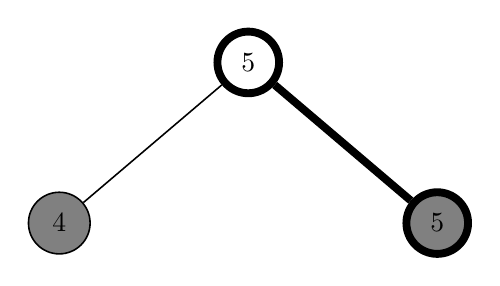
\begin{tikzpicture}[bold, scale=12]
                % The Tree
                \node(0)[max]{5}
                child{node [min, thin]{4} edge from parent[thin]}
                child{node [min]{5}};
            \end{tikzpicture}
        }
    \end{subfigure}
    &
    \begin{subfigure}[b]{0.22\textwidth}
        \centering
        \resizebox{\textwidth}{!}{
            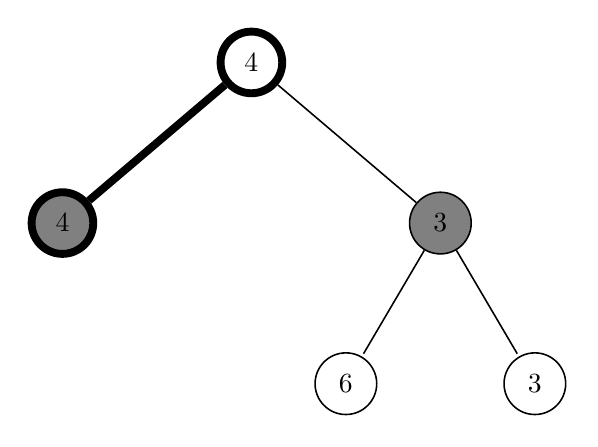
\begin{tikzpicture}[bold, scale=12]
                % The Tree
                \node(0)[max]{4}
                child{node [min]{4}}
                child{node [min, thin]{3}
                    child{node [max] {6}}
                    child{node [max] {3}}
                    edge from parent[thin]
                };
            \end{tikzpicture}
        }
    \end{subfigure}
    &
    \begin{subfigure}[b]{0.22\textwidth}
        \centering
        \resizebox{\textwidth}{!}{
            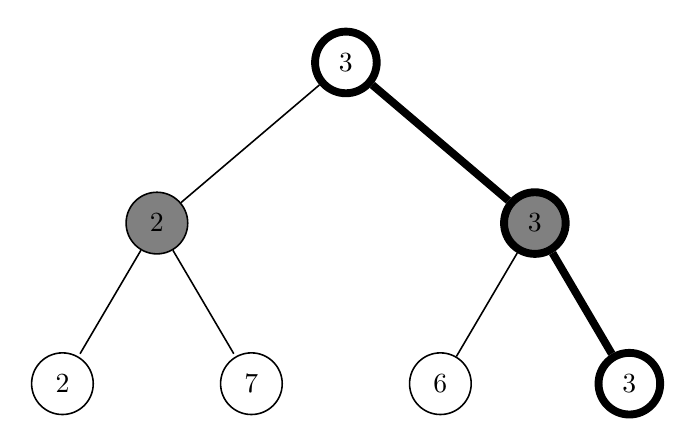
\begin{tikzpicture}[bold, scale=12]
                % The Tree
                \node(0)[max]{3}
                child{node [min, thin]{2}
                    child{node [max] {2}}
                    child{node [max] {7}}
                    edge from parent[thin]
                }
                child{node [min]{3}
                    child{node [max, thin] {6}
                        edge from parent [thin]
                    }
                    child{node [max] {3}}
                };
            \end{tikzpicture}
        }
    \end{subfigure}
    &
    \begin{subfigure}[b]{0.22\textwidth}
        \centering
        \resizebox{\textwidth}{!}{
            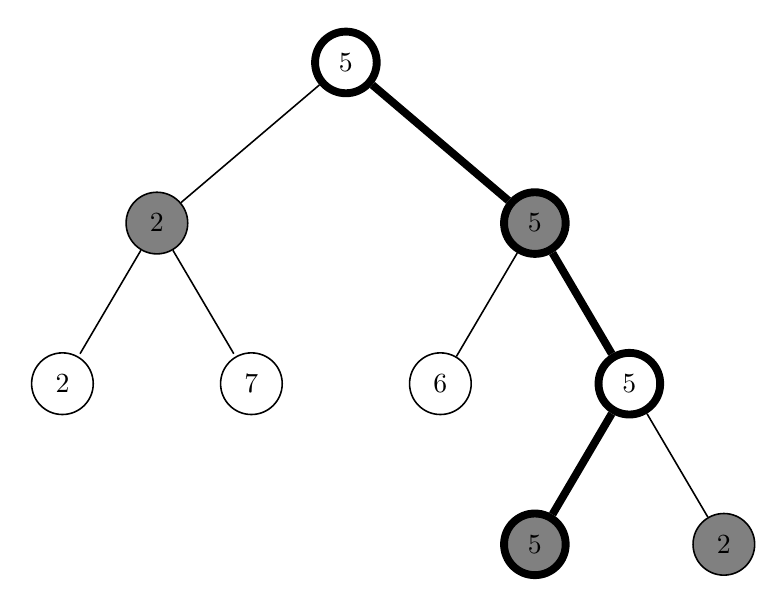
\begin{tikzpicture}[bold, scale=12]
                % The Tree
                \node(0)[max]{5}
                child{node [min, thin]{2}
                    child{node [max] {2}}
                    child{node [max] {7}}
                    edge from parent[thin]
                }
                child{node [min]{5}
                    child{node [max, thin] {6}
                        edge from parent [thin]
                    }
                    child{node [max] {5}
                        child{node [min] {5}}
                        child{node [min, thin] {2}
                            edge from parent [thin]
                        }
                    }
                };
            \end{tikzpicture}
        }
    \end{subfigure}

    \end{tabular}

    \caption{Best first minimax on an example tree. Each iteration expands
    all children of the leaf at the end of the principal variation, and
    backpropagates the new minimax values up the tree.}

    \label{fig:bestfirstminimax}

\end{figure}


\newpage
\subsection{Monte Carlo Tree Search}

Monte Carlo methods in AI rely on information from many simulated games played with randomly selected actions to guide decision making in the current state. In its most basic form, Monte Carlo sampling generates all successors $S'(s)$ of the current state $s$, and simulates multiple games starting from each successor state until the budget runs out. These simulated games are called rollouts, and the budget can either be a fixed number of rollouts, or a time limit. When the budget runs out, the action leading to the successor state with the highest average utility $\hat{U}$ is chosen as the next action.

\begin{figure}[H]
    \centering
    
    \tikzset{
    state/.style={circle,draw,inner sep=5},
    win/.style={circle,draw,inner sep=2},
    loss/.style={circle,draw,inner sep=2, fill=black}
    }
    
    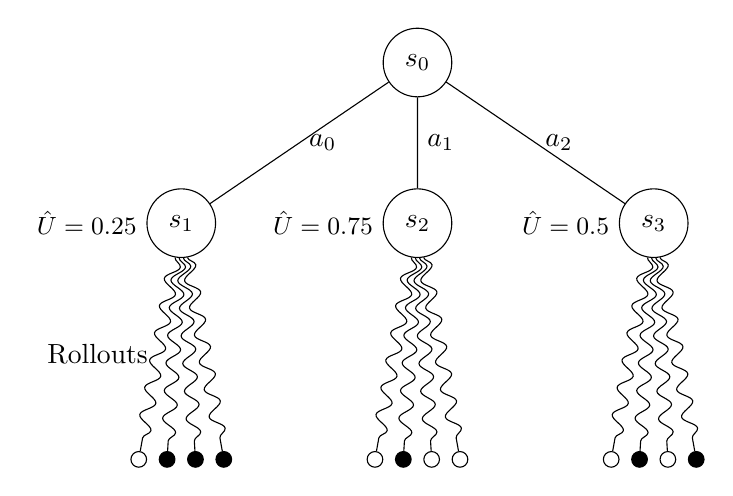
\begin{tikzpicture}[scale=12]
    % Specify spacing for each level of the tree
    \tikzstyle{level 1}=[level distance=1.7mm,sibling distance=2.5mm]
    \tikzstyle{level 2}=[level distance=2.5mm,sibling distance=.3mm]
    % The Tree
    \node(0)[state]{$s_0$}
    child{node[state, label=left:{\small $\hat{U}=0.25$}]{$s_1$}
    child{node[win]{}
        edge from parent[decorate, decoration=snake] node[left]{Rollouts}
        }
        child{node[loss]{}
        edge from parent[decorate, decoration=snake]
        }
        child{node[loss]{}
        edge from parent[decorate, decoration=snake]
        }
        child{node[loss]{}
        edge from parent[decorate, decoration=snake]
        }
        edge from parent node[right]{$a_0$}
    }
    child{node[state, label=left:{\small $\hat{U}=0.75$}]{$s_2$}
        child{node[win]{}
        edge from parent[decorate, decoration=snake]
        }
        child{node[loss]{}
        edge from parent[decorate, decoration=snake]
        }
        child{node[win]{}
        edge from parent[decorate, decoration=snake]
        }
        child{node[win]{}
        edge from parent[decorate, decoration=snake]
        }
        edge from parent node[right]{$a_1$}
    }
    child{node[state, label=left:{\small $\hat{U}=0.5$}]{$s_3$}
        child{node[win]{}
        edge from parent[decorate, decoration=snake]
        }
        child{node[loss]{}
        edge from parent[decorate, decoration=snake]
        }
        child{node[win]{}
        edge from parent[decorate, decoration=snake]
        }
        child{node[loss]{}
        edge from parent[decorate, decoration=snake]
        }
        edge from parent node[right]{$a_2$}
    };

    \end{tikzpicture}

    \caption{The simplest Monte Carlo method, with a budget of 12 total
    rollouts. White leaf nodes
    corresponds to wins, and black to losses. Action $a_1$ maximizes
    the average utility $\hat{U}$ at 0.75, and is therefore the move chosen.}
    \label{fig:simple_monte_carlo}

\end{figure}

The approach in Figure \ref{fig:simple_monte_carlo} chooses which node to sample next in such a way that it keeps the number of simulations for each node balanced. This is a naive approach in the sense that if a state looks very unpromising, it will still take up the same fraction of rollouts as the more promising ones. To formalize the concept of spending time on suboptimal states, the idea of \textit{regret} is introduced. Assuming that each state $s_i$ has a true mean utility $\bar{U}_i$, the maximum mean utility is denoted $U^*$, and its state $s^*$. The regret of performing rollout $n$ from state $s_i$ is then $l_n = U^* - \bar{U}_i$, and the cumulative regret of all rollouts is $L_N = \sum_{n=0}^N l_n$. The goal is then to choose a rollout policy that minimizes $L_N$. Since all states but $s^*$ has positive regret, it is clear that balancing the rollouts evenly between all states will result in $L_N$ being linear in $N$. It can be shown that choosing the next rollout greedily, i.e. choosing the state where $\hat{U}$ is currently largest, also results in linear cumulative regret, even if random exploration is performed with probability $\epsilon$ (knowns as an $\epsilon$-greedy policy).
To improve upon this, Auer and Fischer \cite{Auer2002} utilised the idea of upper condifence bounds, valuing states highly not only if their $\hat{U}$ value is high, but also if the number of rollouts from the state is low. This encourages exploration that still acknowledges $\hat{U}$, and results in cumulative regret that is logarithmic in $N$. Their selection policy chooses the state that maximizes the UCB1 value:

\begin{equation}
    \text{UCB1}(s_i) = \hat{U}_i + 
    c\sqrt{\frac{\log{N}}{n_i}}
\end{equation}

The first term in UCB1 is the exploitation term, and makes sure that the algorithm gravitates toward states with a high utility. The second term is the exploration term, which increases the value of nodes that have not seen many rollouts compared to $N$. This prevents the algorithm from getting stuck on suboptimal nodes in case their initial few rollouts are a bad estimation of their true utility. The parameter $c$ balances the two terms, and a value of $\sqrt{2}$ is theoretically optimal for utilities on $[0, 1]$.

Monte Carlo Tree Search (MCTS) \cite{Coulom2006, Chang2005} expands the classical idea of Monte Carlo sampling by expanding a partial game tree containing the results of the simulations, and using these results to guide further simulations. Nodes in the game tree store the following information:

\begin{itemize}
    \item State: Game state $s \in S$
    \item Count: Number of simulations from this node or its descendants
    \item Utility: Cumulative utility from simulations from this node or its descendants
    \item Parent: The node that generated this node
    \item Children: List of nodes containing successor states
    \item Unexpanded Actions: Actions from $A(s)$ that have not yet been used to generate a successor state 
\end{itemize}

At creation, each nodes unexpanded actions list is initialized
with the applicable actions from its state. To build up the 
game tree, a root node is created containing the 
current game state, and then each iteration of the algorithm goes through 
the steps seen in Algorithm \ref{alg:mcts}:

\begin{figure}[H]
    \centering

    \tikzset{
    max/.style={circle,draw,inner sep=5},
    min/.style={circle,draw,inner sep=5, fill=gray},
    bold/.style={line width=1mm},
    thin/.style={line width=0.2mm}
    }

    % Specify spacing for each level of the tree
    \tikzstyle{level 1}=[level distance=1.7mm,sibling distance=4mm]
    \tikzstyle{level 2}=[level distance=1.7mm,sibling distance=2mm]
    
    \begin{tabular}{cc}
        
    \begin{subfigure}[b]{0.4\textwidth}
        \centering
        \resizebox{\textwidth}{!}{
            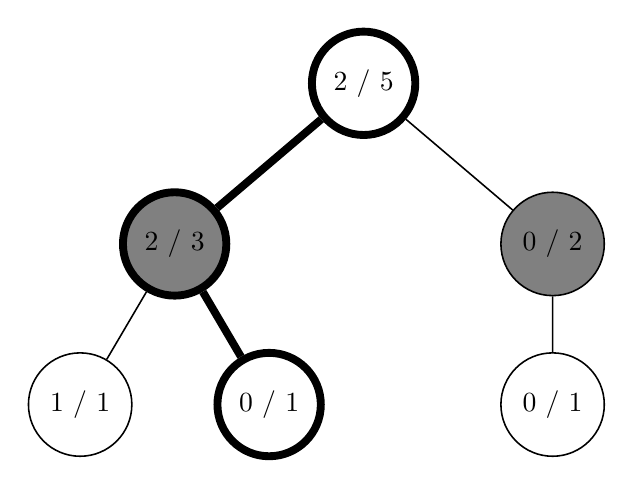
\begin{tikzpicture}[bold, scale=12]
                % The Tree
                \node(0)[max]{2 / 5}
                child{node[min]{2 / 3}
                    child{node[max, thin]{1 / 1} edge from parent[thin]}
                    child{node[max]{0 / 1}}
                }
                child{[thin]node[min]{0 / 2}
                    child{node[max]{0 / 1}}
                };
            \end{tikzpicture}
        }
        \caption*{Selection}
    \end{subfigure}
    &
    \begin{subfigure}[b]{0.4\textwidth}
        \centering
        \resizebox{\textwidth}{!}{
            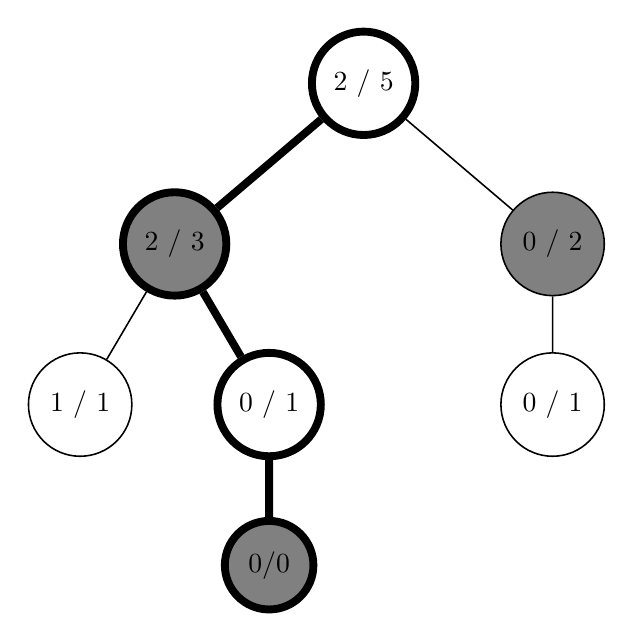
\begin{tikzpicture}[bold, scale=12]
                % The Tree
                \node(0)[max]{2 / 5}
                child{node[min]{2 / 3}
                    child{node[max, thin]{1 / 1} edge from parent[thin]}
                    child{node[max]{0 / 1}
                        child{node[min]{0/0}}
                    }
                }
                child{[thin]node[min]{0 / 2}
                    child{node[max]{0 / 1}}
                };
            \end{tikzpicture}
        }
        \caption*{Expansion}
    \end{subfigure}
    \\
    \begin{subfigure}[b]{0.4\textwidth}
        \centering
        \resizebox{\textwidth}{!}{
            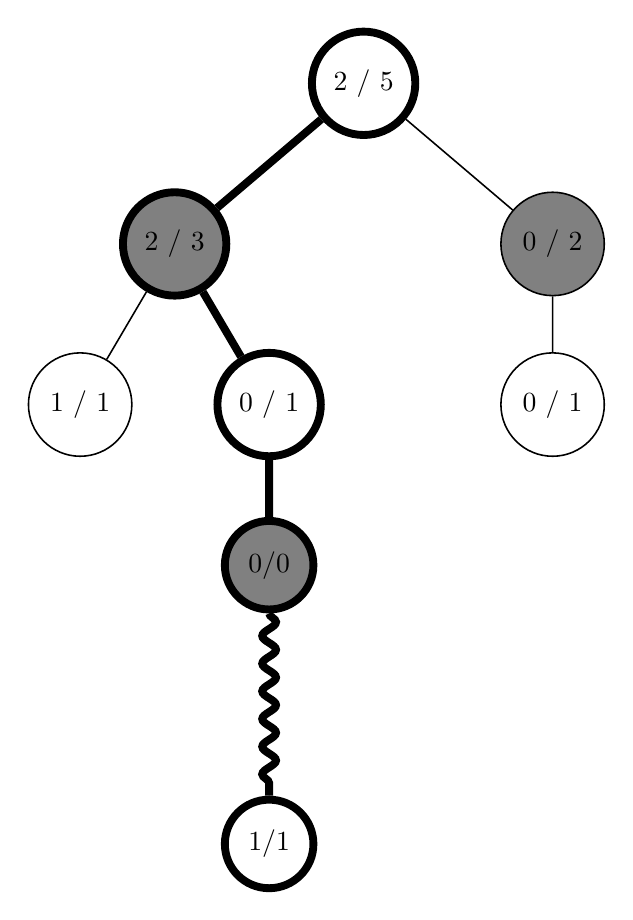
\begin{tikzpicture}[bold, scale=12]
                % The Tree
                \node(0)[max]{2 / 5}
                child{node[min]{2 / 3}
                    child{node[max, thin]{1 / 1} edge from parent[thin]}
                    child{node[max]{0 / 1}
                        child{node[min]{0/0}
                            child{node[max, yshift=-1.5cm]{1/1} edge from parent[decorate, decoration=snake]}
                        }
                    }                }
                child{[thin]node[min]{0 / 2}
                    child{node[max]{0 / 1}}
                };
            \end{tikzpicture}
        }
        \caption*{Simulation}
    \end{subfigure}
    &
    \begin{subfigure}[b]{0.4\textwidth}
        \centering
        \resizebox{\textwidth}{!}{
            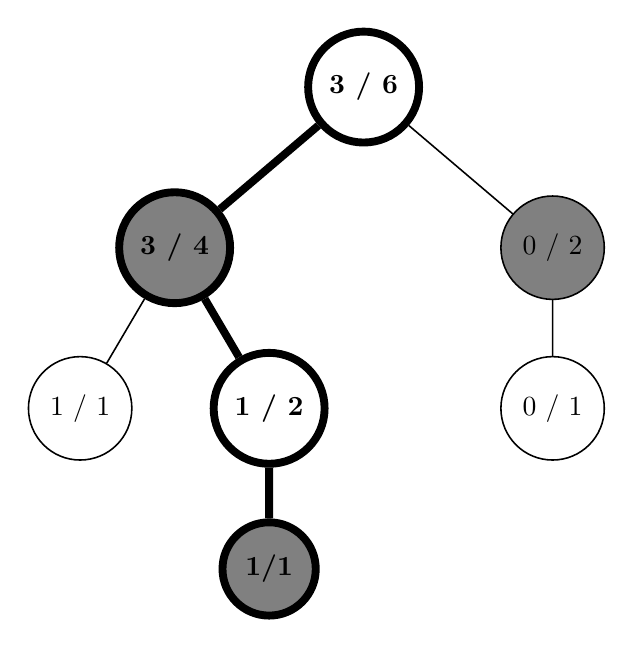
\begin{tikzpicture}[bold, scale=12]
                % The Tree
                \node(0)[max]{\textbf{3 / 6}}
                child{node[min]{\textbf{3 / 4}}
                    child{node[max, thin]{1 / 1} edge from parent[thin]}
                    child{node[max]{\textbf{1 / 2}}
                        child{node[min]{\textbf{1/1}}}
                    }
                }
                child{[thin]node[min]{0 / 2}
                    child{node[max]{0 / 1}}
                };
            \end{tikzpicture}
        }
        \caption*{Backpropagation}
    \end{subfigure}

    \end{tabular}


   
    \caption{One iteration of MCTS on an example graph. Node labels signify utility / count. Note that the count of each non-root node is equal to the sum of the count of its children plus one, since a simulation was also performed when the node was originally expanded. Likewise the utility can be one higher than the sum of child utilities if the simulation was a Max player win.}
    \label{fig:mcts_illustrated}

\end{figure}


\textbf{Select:} The selection step starts in the root of the tree,
and progresses recursively down through the tree using the following
rules: If the current node contains a terminal state, or the node still has unexpanded actions, return the node. Otherwise, run the selection
step again on the child $C$ with the highest $UCB1$ value, where $N$ is set to $C.Parent.Count$. The application of UCB1 on trees is usually called UCT, or Upper Confidence bounds on Trees.
Note that if backpropagation does not take into account the difference
between Max and Min nodes, UCB1 should use a modified exploitation term 
for the Min player. For utilities on the interval $[0,1]$, 
$1 - \frac{Utility}{Count}$ can be used.
\begin{algorithm}
    \begin{algorithmic}[1]
        \Procedure{Select}{Node}
            \If{$\text{Node.State} \in S^\circ$ \textbf{or not} 
            FullyExpanded(Node)}
                \State \Return Node
            \EndIf
            \State Child = 
            $\text{arg}\max \{ \text{UCB1}(c) \;|\; c \in \text{Node.Children} \}$ 
            \State \Return Select(Child)
        \EndProcedure
    \end{algorithmic}        
\end{algorithm}

\textbf{Expand:} In the expansion step, the selected node is expanded by 
popping an action from Unexpanded Actions, and adding a child 
node containing the successor state corresponding to that action. This
child node is then also returned. If the selected node contains a terminal 
state or has no unexpanded actions, the selected node is returned instead.

\begin{algorithm}[H]
    \begin{algorithmic}[1]
        \Procedure{Expand}{Node}
            \If{$\text{Node.State} \in S^\circ$ \textbf{or} 
            FullyExpanded(Node)}        
                \State \Return Node
            \EndIf
            \State Action = Node.UnexpandedActions.Pop()
            \State Leaf = MCTSTreeNode(Result(Node.State, Action))
            \State Node.Children.Append(Leaf)
            \State \Return Leaf
        \EndProcedure
    \end{algorithmic}    
\end{algorithm}


\textbf{Simulate:} Starting from the state in the expanded node, a rollout
is performed. As previously noted, a rollout consists of taking random
actions until a terminal state is reached, and then returning the utility
of that state.

\begin{algorithm}
    \begin{algorithmic}[1]
        \Procedure{Simulate}{Node}
            \State State = Node.State
            \While{\textbf{not} State $\in S^\circ$}
                \State Action = ChooseRandom(A(State))
                \State State = Result(State, Action)
            \EndWhile
            \State \Return U(State)
        \EndProcedure
    \end{algorithmic}    
\end{algorithm}

\textbf{Backpropagate:} Starting at the expanded node, count is 
incremented by $1$, and utility is incremented by the result of
the simulation. If the node is not the root, backpropagation
is then called on the roots parent.

\begin{algorithm}
    \begin{algorithmic}[1]
        \Procedure{Backpropagate}{Leaf, Value}     
            \State Leaf.Utility $\leftarrow$ Leaf.Utility $+$ Value
            \State Leaf.Count $\leftarrow$ Leaf.Count $+$ 1
            \If{Leaf.Parent}        
                \State Backpropagate(Leaf.Parent, Value)
            \EndIf
        \EndProcedure
    \end{algorithmic}    
\end{algorithm}

Usually the backpropagation step differentiates between Max and Min nodes, and assigns utilities accordingly. Since the Max nodes have Min nodes as children and has to maximize over those, it is the Min nodes that recieve $+1$ if the Max player wins, and vice versa. In this paper the responsibility of differentiating between node types is delegated to the selection step, partly because it makes the average utilities more compatible with methods introduced later, and partly because it is arguably more intuitive. To see all the steps illustrated, see Figure \ref{fig:mcts_illustrated}.

\begin{figure}[H]
    \centering

    \tikzset{
    max/.style={circle,draw,inner sep=5},
    min/.style={circle,draw,inner sep=5, fill=gray},
    bold/.style={line width=1mm},
    thin/.style={line width=0.2mm}
    }

    % Specify spacing for each level of the tree
    \tikzstyle{level 1}=[level distance=1.7mm,sibling distance=4mm]
    \tikzstyle{level 2}=[level distance=1.7mm,sibling distance=2mm]
    
    \begin{tabular}{cc}
        
    \begin{subfigure}[b]{0.4\textwidth}
        \centering
        \resizebox{\textwidth}{!}{
            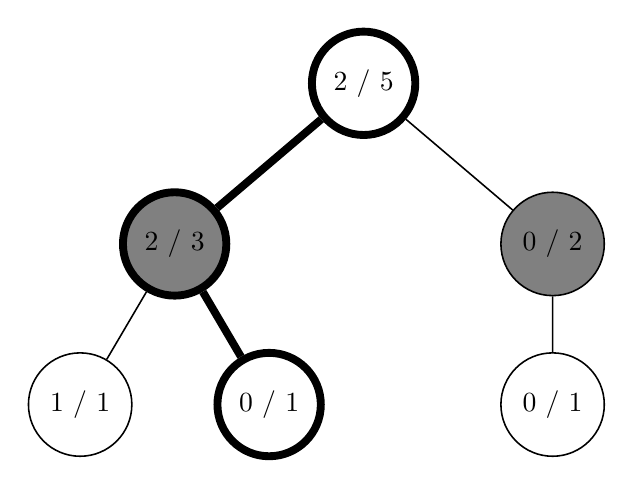
\begin{tikzpicture}[bold, scale=12]
                % The Tree
                \node(0)[max]{2 / 5}
                child{node[min]{2 / 3}
                    child{node[max, thin]{1 / 1} edge from parent[thin]}
                    child{node[max]{0 / 1}}
                }
                child{[thin]node[min]{0 / 2}
                    child{node[max]{0 / 1}}
                };
            \end{tikzpicture}
        }
        \caption*{Selection}
    \end{subfigure}
    &
    \begin{subfigure}[b]{0.4\textwidth}
        \centering
        \resizebox{\textwidth}{!}{
            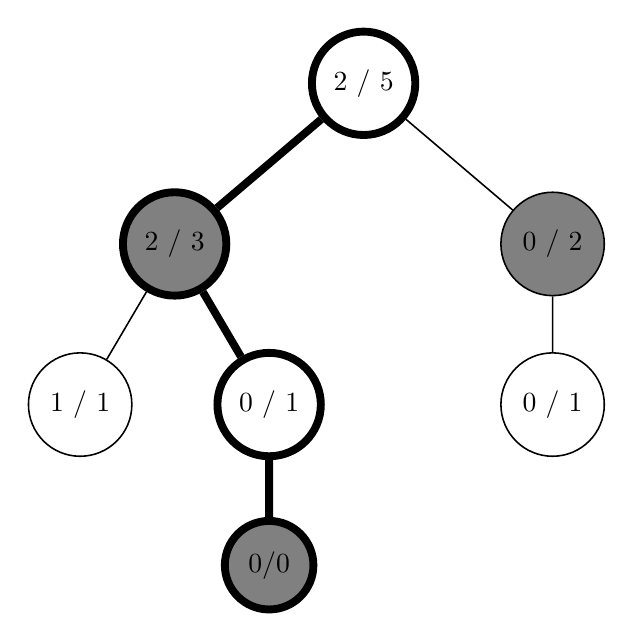
\begin{tikzpicture}[bold, scale=12]
                % The Tree
                \node(0)[max]{2 / 5}
                child{node[min]{2 / 3}
                    child{node[max, thin]{1 / 1} edge from parent[thin]}
                    child{node[max]{0 / 1}
                        child{node[min]{0/0}}
                    }
                }
                child{[thin]node[min]{0 / 2}
                    child{node[max]{0 / 1}}
                };
            \end{tikzpicture}
        }
        \caption*{Expansion}
    \end{subfigure}
    \\
    \begin{subfigure}[b]{0.4\textwidth}
        \centering
        \resizebox{\textwidth}{!}{
            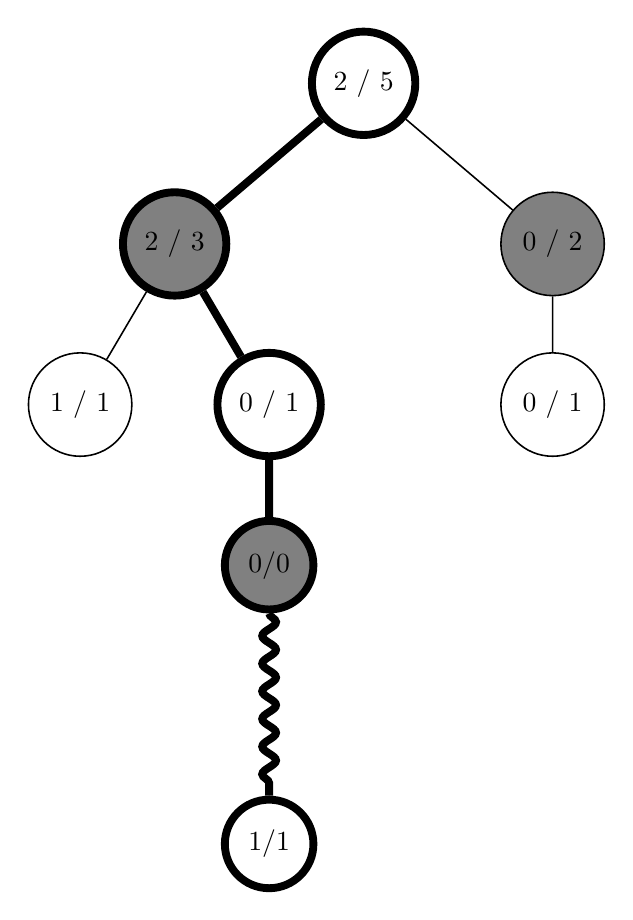
\begin{tikzpicture}[bold, scale=12]
                % The Tree
                \node(0)[max]{2 / 5}
                child{node[min]{2 / 3}
                    child{node[max, thin]{1 / 1} edge from parent[thin]}
                    child{node[max]{0 / 1}
                        child{node[min]{0/0}
                            child{node[max, yshift=-1.5cm]{1/1} edge from parent[decorate, decoration=snake]}
                        }
                    }                }
                child{[thin]node[min]{0 / 2}
                    child{node[max]{0 / 1}}
                };
            \end{tikzpicture}
        }
        \caption*{Simulation}
    \end{subfigure}
    &
    \begin{subfigure}[b]{0.4\textwidth}
        \centering
        \resizebox{\textwidth}{!}{
            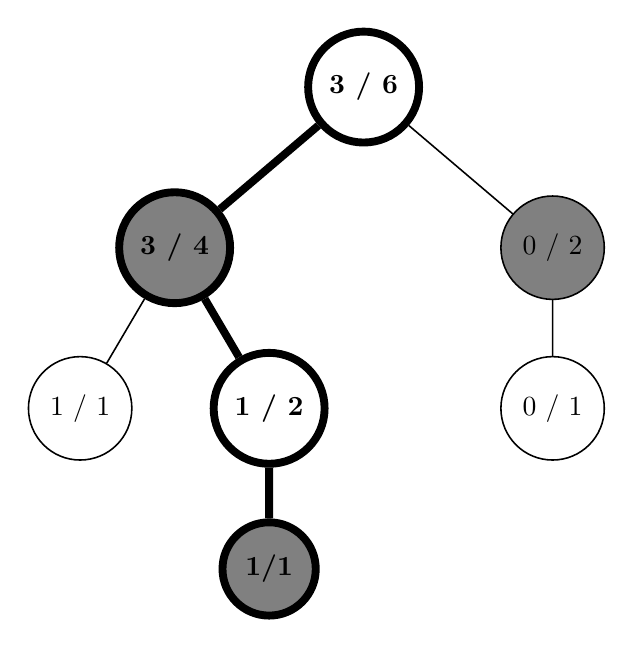
\begin{tikzpicture}[bold, scale=12]
                % The Tree
                \node(0)[max]{\textbf{3 / 6}}
                child{node[min]{\textbf{3 / 4}}
                    child{node[max, thin]{1 / 1} edge from parent[thin]}
                    child{node[max]{\textbf{1 / 2}}
                        child{node[min]{\textbf{1/1}}}
                    }
                }
                child{[thin]node[min]{0 / 2}
                    child{node[max]{0 / 1}}
                };
            \end{tikzpicture}
        }
        \caption*{Backpropagation}
    \end{subfigure}

    \end{tabular}


   
    \caption{One iteration of MCTS on an example graph. Node labels signify utility / count. Note that the count of each non-root node is equal to the sum of the count of its children plus one, since a simulation was also performed when the node was originally expanded. Likewise the utility can be one higher than the sum of child utilities if the simulation was a Max player win.}
    \label{fig:mcts_illustrated}

\end{figure}


\subsubsection{Partial Expansion}
The base version of MCTS is forced to fully expand a node
before any of its children can be explored. Sometimes however
it may be more worthwile to continue exploring deeper into the
tree immediately. To determine when this is the case, partial
expansion \cite{Jacobsen2014, Frydenberg2015} introduces an upper confidence bound $\text{UCB}_c$ on 
the reward of expanding a new child:

\begin{equation}
    \label{eq:upper_confidence_child}
    \text{UCB}_c(\text{Node}) = 0.5 + \sqrt{\frac{\ln\text{Node.Count}}{1 + |\text{Node.Children}|}}
\end{equation}            

If the node is not fully expanded, partial expansion checks if
$\text{UCB}_c$ is larger than the maximum UCB1 of its children.
If it is, the node is returned for expansion, otherwise selection 
is called on the child with the maximum UCB1:
\begin{algorithm}
    \caption{Partial Expansion MCTS Select}
    \begin{algorithmic}[1]
        \Procedure{Select}{Node}
            \If{$\text{Node.State} \in S^\circ$}
                \State \Return Node
            \EndIf
            \If{$\text{UCB}_c(\text{Node}) > \max \{ \text{UCB1}(c) \;|\; c \in \text{Node.Children} \}$ \textbf{and not} FullyExpanded(Node)}
            \State \Return Node
            \Else
            \State Child = 
            $\text{arg}\max \{ \text{UCB1}(c) \;|\; c \in \text{Node.Children} \}$ 
            \State \Return \textproc{Select}(Child)

            \EndIf
        \EndProcedure
    \end{algorithmic}        
\end{algorithm}